%!TeX root=../tese.tex
\chapter{Restrições de grau mínimo}
\label{cap:grau-limitado}

% ---------------------------------------
% ------- Vibe coding começa aqui -------
% ---------------------------------------

% Comando personalizado para desenhar o grafo de Andrásfai com parâmetro d
\newcommand{\drawAndrasfai}[1]{%
  \def\d{#1}                              % parâmetro d
  \pgfmathsetmacro\n{int(3*\d - 1)}       % número de vértices n = 3d - 2
  \begin{tikzpicture}[scale=1.4,
    every node/.style={circle, draw, fill=white, inner sep=1pt, font=\small}]
  
  % 1. Coloca os vértices uniformemente em círculo
  \foreach \i in {0,...,\numexpr \n-1 \relax} {
    \pgfmathsetmacro\angle{90-360*\i/\n}
    \node (v\i) at (\angle:1) {\i};       % vértice v_i na posição angular correspondente
  }

  % 2. Para cada vértice, conecta aos d vértices mais distantes
  \foreach \i in {0,...,\numexpr \n-1 \relax} {
    \foreach \offset in {0,...,\numexpr \d-1 \relax} {
      \pgfmathsetmacro\j{mod(\i + \d + \offset, \n)} % vértice mais distante no ciclo
      \pgfmathtruncatemacro{\ii}{\i}
      \pgfmathtruncatemacro{\jj}{\j}
      \ifnum\ii<\jj
        \draw (v\ii) -- (v\jj);          % desenha aresta se ii < jj (para evitar duplicação)
      \fi
    }
  }

  \end{tikzpicture}
}

% --------------------------------------
% ------ Vibe coding termina aqui ------
% --------------------------------------

\newcommand{\homarrow}{\hookrightarrow}

\section{Grafos livres de triângulos com grau mínimo alto}

Na literatura que trata da Teoria Extremal dos Grafos, o estudo de grafos livres de certos subgrafos com grau mínimo limitado inferiormente merece atenção especial.
Um dos teoremas mais fundamentais nesse sentido é o seguinte teorema de Andrásfai, Erd\H os e Sós:
\begin{theorem}[\cite{andrasfai19742n5}]\label{thm:a-e-s}
  Seja $r \geq 2$ e $G$ um grafo livre de $K_{r+1}$ com $n$ vértices.
  Se \[\delta(G) > \frac{3r-4}{3r-1}n,\]
  então $G$ é $r$-partido.
\end{theorem}

Para grafos livres de triângulos, o Teorema~\ref{thm:a-e-s} prova que, se um grafo livre de triângulos tem grau mínimo maior que $\delta(G) > 2n/5$, então ele é bipartido.
Automaticamente, a Conjectura~\ref{conj:make-bipartite} é verdadeira para grafos com grau mínimo maior que $2n/5$.
Mas se $\delta(G) > 2n/5$, então $e(G) > n^2/5$, o que já é coberto pelo Teorema~\ref{thm:n2/5}.
Portanto, é de se perguntar se a condição de grau mínimo pode ser relaxada, a fim de obter algum resultado que não seja trivial dada a restrição $e(G) \geq n^2/5$.

Para obter esse relaxamento, usamos o seguinte importante resultado:
\begin{theorem}[\cite{brandt2011vega}]~\label{thm:brandt-thomasse}
  Seja $G$ um grafo livre de triângulos com $n$ vértices e $\delta(G) > n/3$.
  Então $G$ é homomórfico a um grafo Vega.
\end{theorem}
%Além disso, o resultado de~\cite{brandt2011vega} permite caracterizar completamente os grafos livres de triângulos e grau mínimo maior que $n/3$ como os grafos homomórficos aos \emph{grafos Vega}.
Não definimos precisamente os grafos Vega porque não os utilizaremos de forma direta no trabalho (o menor deles tem $11$ vértices).
Por ora, é suficiente dizer que os grafos Vega são supergrafos dos grafos de Andrásfai que apresentaremos em breve, e veremos que, com condições levemente relaxadas, o Teorema~\ref{thm:brandt-thomasse} possui análogos mais simples em termos de grafos de Andrásfai.

É interessante observar que a condição do Teorema~\ref{thm:brandt-thomasse} não pode ser substituída por $\delta(G) > cn$ para nenhum $c < 1/3$.
De fato, para todo $\varepsilon > 0$, existem grafos de $n$ vértices com grau mínimo maior que $(1/3-\varepsilon)n$ mas número cromático não limitado (ver~\cite{erdos1973valence}).

%O Teorema~\ref{thm:brandt-thomasse} permite descrever exatamente quem são os conjuntos de arestas que podemos remover para calcular $D(G)$ sempre que $\delta(G)>n/3$ usando o Teorema~\ref{thm:simetrizacao}.
%Porém, a estrutura dos grafos Vega é não-trivial (o menor deles tem 11 vértices), e por isso iremos restringir a nossa análise a um teorema estrutural mais simples com a restrição adicional de $\chi(G)=3$ ou a restrição de grau mínimo substituída por $\delta(G) > 10n/29$.

De toda forma, a utilidade do Teorema~\ref{thm:brandt-thomasse} e de teoremas de homomorfismo relacionados é que, se temos um teorema que garante que $G$ com uma quantidade muito grande de vértices é homomórfico a $H$ (que tem, digamos, $8$ vértices), então pelo Teorema~\ref{thm:simetrizacao} sabemos exatamente como proceder para encontrar candidatos de conjuntos de arestas que, removidos, podem realizar $D(G)$.

\subsection{Grafos de Andrásfai}

Os grafos de Andrásfai são importantes estruturas no estudo de propriedade de estabilidade em grafos livres de triângulos e são definidos da seguinte forma.
\begin{definition}
  Seja $d \geq 1$ um inteiro positivo.
  O \emph{grafo de Andrásfai} $F_d$ é o grafo com vértices $\{0,1,\dots,3d-2\}$ (vistos módulo $3d-1$) e arestas entre $i$ e $i+d+j$ para cada $i \in \{0,1,\dots,3d-2\}$ e cada $j \in \{0,1,\dots,d-1\}$.
\end{definition}
Uma forma de representar os grafos de Andrásfai é colocar os vértices em uma circunferência em sentido horário como vértices de $(3d-1)$-ágono regular e ligar cada vértice com os $d$ vértices mais distantes.

\begin{figure}[htbp]
  \centering

  \begin{subfigure}[b]{0.22\textwidth}
    \centering
    \drawAndrasfai{1}
    \caption*{$F_1$}
  \end{subfigure}
  \hfill
  \begin{subfigure}[b]{0.22\textwidth}
    \centering
    \drawAndrasfai{2}
    \caption*{$F_2$}
  \end{subfigure}
  \hfill
  \begin{subfigure}[b]{0.22\textwidth}
    \centering
    \drawAndrasfai{3}
    \caption*{$F_3$}
  \end{subfigure}
  \hfill
  \begin{subfigure}[b]{0.22\textwidth}
    \centering
    \drawAndrasfai{4}
    \caption*{$F_4$}
  \end{subfigure}

  \caption{Grafos de Andrásfai para $d \in \{1,2,3,4\}$. Observe que $F_d$ é $d$-regular e livre de triângulos.}
\end{figure}

%No que se segue, para grafos $G$ e $H$, usaremos a notação $G \homarrow H$ para representar que $G$ é homomórfico a $H$ (isto é, $G$ é um subgrafo de um blow-up de $H$).
Os Teoremas~\ref{thm:jin} e~\ref{thm:hom-to-Fd} formam a caracterização estrutural que estamos procurando.

\begin{theorem} [\cite{jin199510n29}] \label{thm:jin}
  Seja $G$ um grafo livre de triângulos com $n$ vértices e grau mínimo maior que $10n/29$.
  Então $G \homarrow F_9$.
\end{theorem}

\begin{theorem} [\cite{chen1997triangle}] \label{thm:hom-to-Fd}
  Seja $G$ um grafo livre de triângulos com $n$ vértices e $\chi(G) \leq 3$.
  Se $\delta(G) > \frac{d+1}{3d+2}n$ para algum $d \geq 1$, então $G \homarrow F_d$.
\end{theorem}

Do Teorema~\ref{thm:hom-to-Fd}, segue diretamente que se $G$ é um grafo livre de triângulos com $n$ vértices satisfazendo $\delta(G) > n/3$ e $\chi(G) \leq 3$, então $G$ é homomórfico a algum $F_d$.

\section{A Conjectura~\ref{conj:make-bipartite} para grafos de Andrásfai}

Em~\cite{mota2019andrasfai}, os autores verificam o seguinte resultado para a Conjectura~\ref{conj:metadinha}:

\begin{theorem}[\cite{mota2019andrasfai}]
  Se um grafo $G$ com $n$ vértices é homomórfico a um grafo de Andrásfai $F_d$ para algum $d \geq 1$, então existe $X \subseteq V(G)$ com $|X| \leq \lfloor n/2 \rfloor$ e $e(G[X]) \leq n^2/50$.
\end{theorem}
Para isso, os autores utilizaram uma representação geométrica de grafos de Andrásfai como subgrafos finitos de um grafo infinito com vértices no círculo unitário, e o conjunto $X$ é escolhido também de forma geométrica, como pontos em um intervalo no círculo com os vértices de $G$.

Inspirados nessa interpretação geométrica de grafos de Andrásfai, provamos o seguinte resultado nessa seção:
\begin{theorem}\label{thm:conds}
  Seja $G$ um grafo livre de triângulos isomorfo a $F_d$ para algum $d \geq 1$.
  Então $G$ satisfaz a Conjectura~\ref{conj:make-bipartite} se alguma das condições abaixo vale:
  \begin{enumerate}
    \item $d \leq 3$; \label{cond:cond-1}
    \item Cada uma das $3d-1$ classes de $G$ tem tamanho no máximo $\tfrac{2}{5d}|G|$. \label{cond:cond-2}
  \end{enumerate}
\end{theorem}

\subsection{Condição~\ref{cond:cond-1}}
\label{sub:cond-1}

Inicialmente, verificamos um lema geral sobre partições do conjunto de arestas em grafos livres de triângulos.

\begin{lemma} \label{lem:odd-transversal}
  Seja $G$ um grafo e suponha que existem $E_1,E_2,E_3,E_4,E_5 \subseteq E$, dois a dois disjuntos, tais que
  $G-E_i$ é bipartido para cada $i \in \{1,2,3,4,5\}$.
  Então $G$ satisfaz a Conjectura \ref{conj:make-bipartite}.
\end{lemma}

\begin{proof}
  Se $e(G) \geq n^2/5$, então o resultado segue do Teorema \ref{thm:n2/5}.
  Por outro lado, se $e(G) < n^2/5$, então
    \[ 5 \min\{ |E_1|,|E_2|,|E_3|,|E_4|,|E_5| \} \leq |E_1|+|E_2|+|E_3|+|E_4|+|E_5| \leq e(G) < \frac{n^2}{5}, \]
  e para $|E_i| = \min \{ |E_1|,|E_2|,|E_3|,|E_4|,|E_5| \}$ temos $G-E_i$ bipartido com $|E_i| < n^2/5$.
\end{proof}

Dessa forma, se apresentarmos uma tal partição para $F_d$, ela também valerá para qualquer blow-up de $F_d$, independentemente dos tamanhos relativos entre as classes no blow-up.
A figura a seguir mostra que tal partição existe para $F_3$, em que cada cor está associada a um $E_i$:

\begin{figure}[htbp]
  \begin{center}
    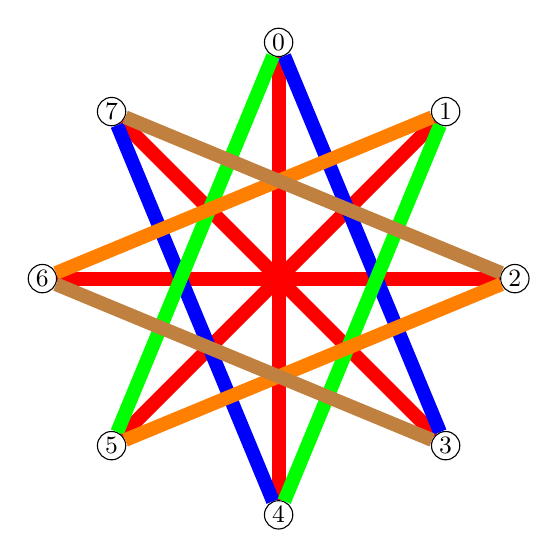
\begin{tikzpicture}[scale=3,
      every node/.style={circle, draw, fill=white, inner sep=1pt, font=\small}]
    
    % 1. Coloca os vértices uniformemente em círculo
    \foreach \i in {0,...,7} {
      \pgfmathsetmacro\angle{90-360*\i/8}
      \node (v\i) at (\angle:1) {\i};       % vértice v_i na posição angular correspondente
    }

    \draw [line width = 5pt, red] (v0)--(v4);
    \draw [line width = 5pt, red] (v1)--(v5);
    \draw [line width = 5pt, red] (v2)--(v6);
    \draw [line width = 5pt, red] (v3)--(v7);

    \draw [line width = 5pt, blue] (v0)--(v3);
    \draw [line width = 5pt, blue] (v7)--(v4);

    \draw [line width = 5pt, green] (v1)--(v4);
    \draw [line width = 5pt, green] (v0)--(v5);

    \draw [line width = 5pt, orange] (v1)--(v6);
    \draw [line width = 5pt, orange] (v2)--(v5);

    \draw [line width = 5pt, brown] (v3)--(v6);
    \draw [line width = 5pt, brown] (v2)--(v7);

    \end{tikzpicture}
  \end{center}
\end{figure}

%O seguinte resultado é imediato da partição acima e dos Teoremas~\ref{thm:jin} e~\ref{thm:hom-to-Fd}.
\begin{corollary}
  Se $G$ é livre de triângulos e $\delta(G)>4n/11$, então $G$ satisfaz a Conjectura~\ref{conj:make-bipartite}.
\end{corollary}
%\begin{proof}
%  Veja que $4/11 > 10/29$, logo pelo Teorema \ref{thm:jin}, temos que $G \homarrow F_9$.
%  Em particular, $\chi(G) \leq \chi(F_9) = 3$.
%  Assim, pelo Teorema \ref{thm:hom-to-Fd} com $d=3$, vale que $G \homarrow F_4$.
%  Considere a seguinte partição das arestas de $G$, em que cada classe está representada por um vértice e todos as arestas entre o mesmo par de classes estão na mesma parte:

Apesar disso, não é fácil generalizar a estratégia de partição de $E(G)$ do Lema~\ref{lem:odd-transversal}, porque essa propriedade não ocorre em geral em grafos de triângulos.
De fato, é fácil verificar que essa partição não existe para $F_4$ e, portanto, não existe para nenhum $F_d$ com $d \geq 4$.


\subsection{Condição~\ref{cond:cond-2}}
\label{sub:cond-2}

Na Seção~\ref{sub:cond-1}, utilizamos a estratégia de tentar encontrar conjuntos explícitos de arestas $F \subseteq E(F_d)$ tais que $F_d - F$ é bipartido e transferir as propriedades dessas arestas para blow-ups de $F_d$.
Pelo Teorema~\ref{thm:simetrizacao}, essa estratégia não é somente razoável, mas suficiente para encontrar conjuntos de arestas de grafos $H \homarrow F_d$ que realizem $D(H)$.

Assim, seguimos a estratégia geral de procurar, em $F_d$, conjuntos de arestas pequenos cuja remoção torna $F_d$ bipartido.
É fácil ver que os conjuntos independentes maximais de $F_d$ são conjuntos de vértices consecutivos (módulo $3d-1$), e portanto é natural considerar conjuntos que possuem a maior quantidade possível de vértices consecutivos, ou seja, com uma das partes tendo os vértices de $0$ a $\lfloor3d/2\rfloor-1$ e a outra parte tendo os vértices de $\lfloor 3d/2 \rfloor$ a $3d-1$.

%\begin{theorem}
%  Seja $d \geq 1$.
%  Então
%  \[ D(F_d) = \left\lfloor\frac{d^2}{4}\right\rfloor. \]
%\end{theorem}

\begin{theorem}
  Seja $d \geq 1$.
  Então \[ D(F_d) \leq \left\lfloor \frac{d^2}{4} \right\rfloor. \]
\end{theorem}

\begin{proof}
Basta apresentar uma bipartição $\{A, B\}$ de $F_d$ com $e(G[A]), e(G[B]) = \lfloor d^2/4 \rfloor$.
Considere a seguinte bipartição $V(F_d) = A \cup B$ em que cada parte é formada por (aproximadamente) metade dos vértices de $F_d$:
\[ V(G) = \{0,1,\dots,\lfloor (3d-1)/2\rfloor -1\} \cup \{3d-2,3d-3,\dots,\lfloor (3d-1)/2\rfloor\}.\]

\begin{figure}[htbp]
  \centering
  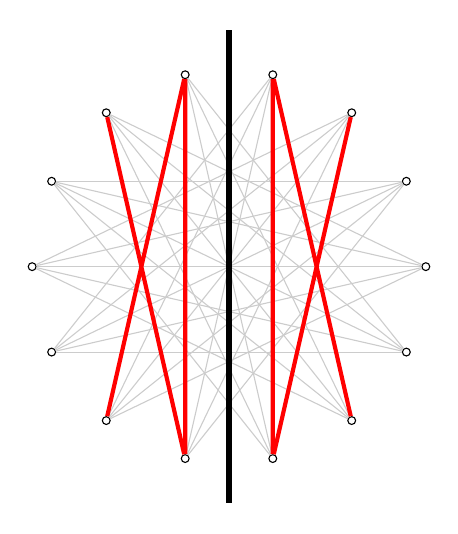
\begin{tikzpicture}[scale=2.5,
    every node/.style={circle, draw, fill=white, inner sep=1pt, font=\small}]
  
  % 1. Coloca os vértices uniformemente em círculo
  \foreach \i in {0,...,13} {
    \pgfmathsetmacro\angle{90-360*\i/14+360/28}
    \node (v\i) at (\angle:1) {};       % vértice v_i na posição angular correspondente
  }

  % 2. Para cada vértice, conecta aos d vértices mais distantes
  \foreach \i in {0,...,13} {
    \foreach \offset in {0,...,4} {
      \pgfmathsetmacro\j{mod(\i + 5 + \offset, 14)} % vértice mais distante no ciclo
      \pgfmathtruncatemacro{\ii}{\i}
      \pgfmathtruncatemacro{\jj}{\j}
      \ifnum\ii<\jj
        \draw[black!20] (v\ii) -- (v\jj);          % desenha aresta se ii < jj (para evitar duplicação)
      \fi
    }
  }

  \draw[red, line width = 1.5pt] (v2) -- (v7) -- (v1) -- (v6);
  \draw[red, line width = 1.5pt] (v9) -- (v0) -- (v8) -- (v13);
  \draw[line width = 2pt] (0,1.2) -- (0,-1.2);
  \end{tikzpicture}
  \caption{Exemplo da bipartição para $d=5$.}
\end{figure}

Em $A$, as arestas que ligam vértices a uma distância $\ell$ (percorrida no círculo no sentido mais próximo) são $\lfloor (3d-1)/2 \rfloor- \ell$, para cada $\ell \in \{d,d+1,\dots,|A|-1\}$.
Fazendo a contagem análoga para $B$, obtemos:
\begin{align*}
  e(G[A])+e(G[B])
  &= \sum_{\ell = d}^{\left\lfloor\frac{3d-1}{2}\right\rfloor-1} \left\lfloor\frac{3d-1}{2}\right\rfloor-\ell + \sum_{\ell = d}^{\left\lceil\frac{3d-1}{2}\right\rceil-1} \left\lceil\frac{3d-1}{2}\right\rceil-\ell \\
  &= \sum_{i=1}^{\left\lfloor\frac{d-1}{2}\right\rfloor}i+\sum_{i=0}^{\left\lceil\frac{d-1}{2}\right\rceil}i \\
  &= \frac12\left(\left\lfloor\frac{d-1}{2}\right\rfloor\left\lfloor\frac{d+1}{2}\right\rfloor+\left\lceil\frac{d-1}{2}\right\rceil\left\lceil\frac{d+1}{2}\right\rceil\right).
\end{align*}
Se $d$ é ímpar, temos $e(G[A])+e(G[B])=2(d^2-1)/8=\lfloor d^2/4 \rfloor$.
Se $d$ é par, temos $e(G[A])+e(G[B])=2d^2/8=\lfloor d^2/4 \rfloor$.

\end{proof}

Finalmente, se toda classe de $G$ tem tamanho no máximo $2|G|/5d$, segue que
\[ D(G) \leq D(F_d) \cdot \frac{4|G|^2}{25d^2} \leq \frac{d^2}{4} \cdot \frac{4|G|^2}{25d^2} = \frac{|G|^2}{25}. \]

O resultado de~\ref{cond:cond-2} pode ser melhorado utilizando os mesmos conjuntos de arestas mas tomando conjuntos de vértices gerados rotacionando a linha que separa as partes do subgrafo bipartido final.
No geral, desejamos incluir pesos $x_0,x_1,\dots,x_{3d-2} \in [0,1]$ com $\sum_{i=0}^{3d-2} x_i = 1$ e modelar o número de arestas removidas como uma expressão da forma $\sum_{ij \in F} x_ix_j$, em que $F \subseteq E(F_d)$ é tal que $F_d - F$ é bipartido.

Contudo, a região factível do programa resultante não é côncava.
Uma forma fácil de verificar isso é tomando $U \subseteq V(F_d)$ tal que $G[U]$ é isomórfico a $C_5$ e a atribuição
\[ \begin{cases}
  x_v = \frac{1}{5} & \text{se } v \in U, \\
  x_v = 0 & \text{se } v \not\in U.
\end{cases} \]
Essa atribuição equivale a um blow-up de $F_d$ que também é um blow-up balanceado de $C_5$, e que não pode ser tornado bipartido pela deleção de menos que $n^2/5$ arestas.
Dessa forma, se a Conjectura~\ref{conj:make-bipartite} for verdadeira, todas essas atribuições são extremos locais para os problemas de otimização razoáveis que podem ser considerados.
Para $d$ pequeno, verificamos empiricamente que, de fato, esses são os únicos extremos locais.